% Source: ANA_EXOT_2025_06_INT1/figures/appendix/ZVR/, Appendix D, Figures D.1--D.2.
% Thesis PDFs: scripts/ch8/prepare_fake_tau_appendix.py removes the ATLAS Internal label visually.
% Verification: output/ch8/fake_appendix_20260925/figure_label_verification.json.
\begin{figure}[htpb]
    \centering
    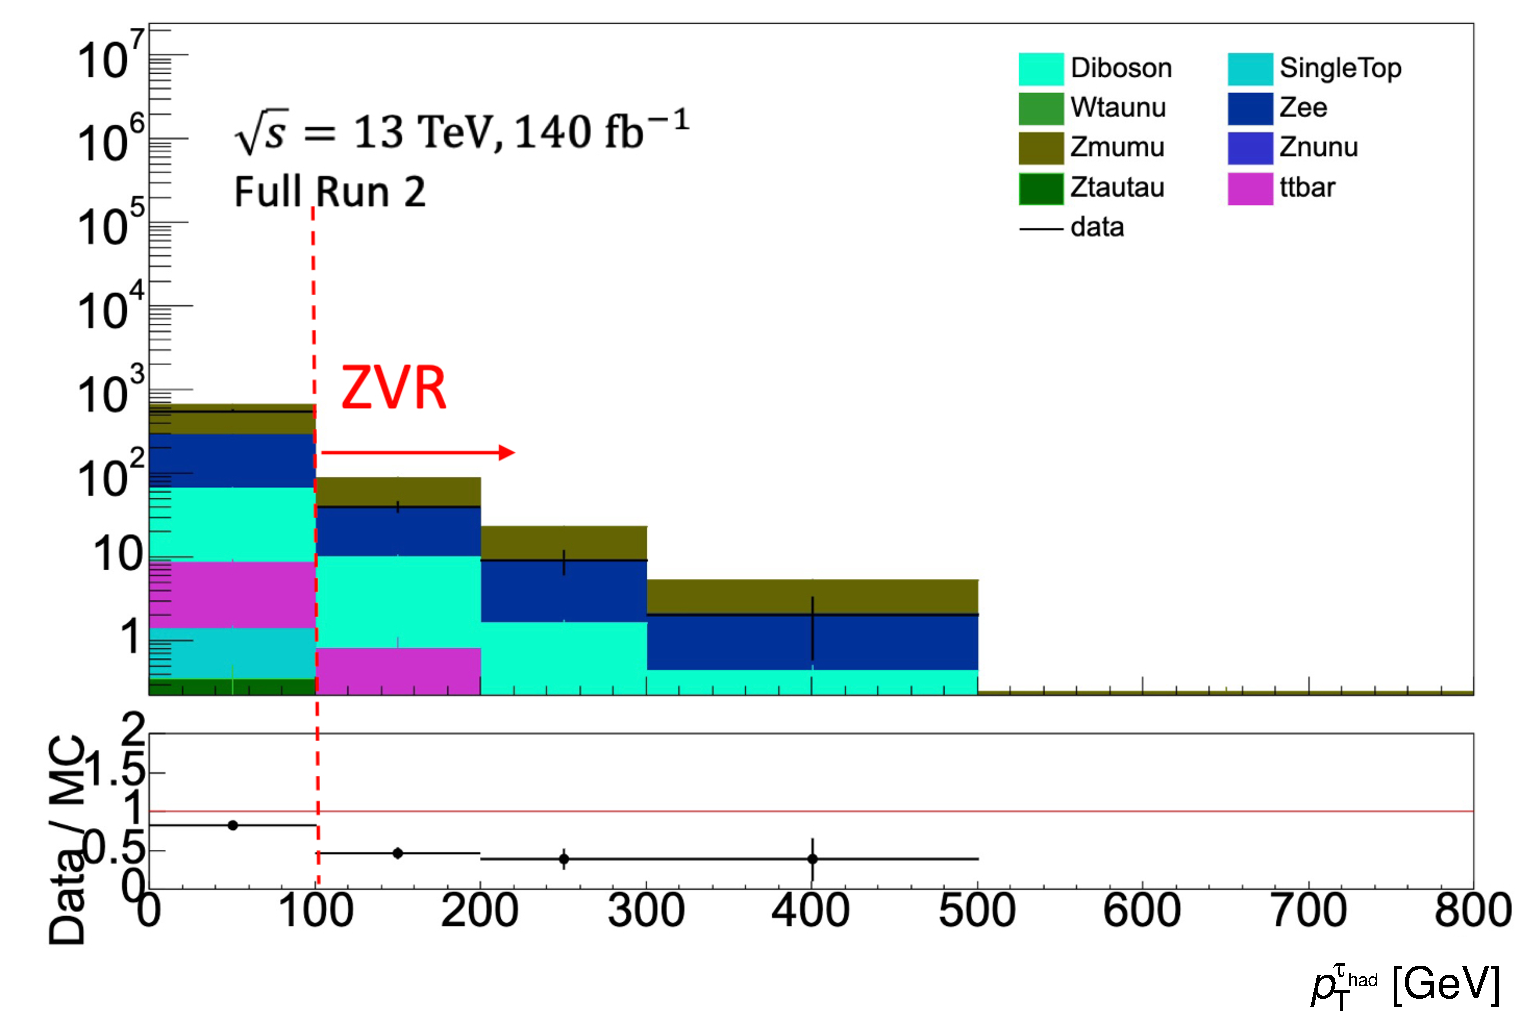
\includegraphics[width=0.80\linewidth]{Figs/CH8/fake_tau_appendix/ZVR_pTtau.pdf}
    \caption[Tau momentum distribution in the ZVR]{$N-1$ kinematic plot of $\pT^{\hadtau}$ in the ZVR. The mismodelling of fake $\hadtau$ in the tail region is observed.}
    \label{fig:ch8_zvr_pt}
\end{figure}

\begin{figure}[htpb]
    \centering
    \begin{subfigure}{0.49\linewidth}
        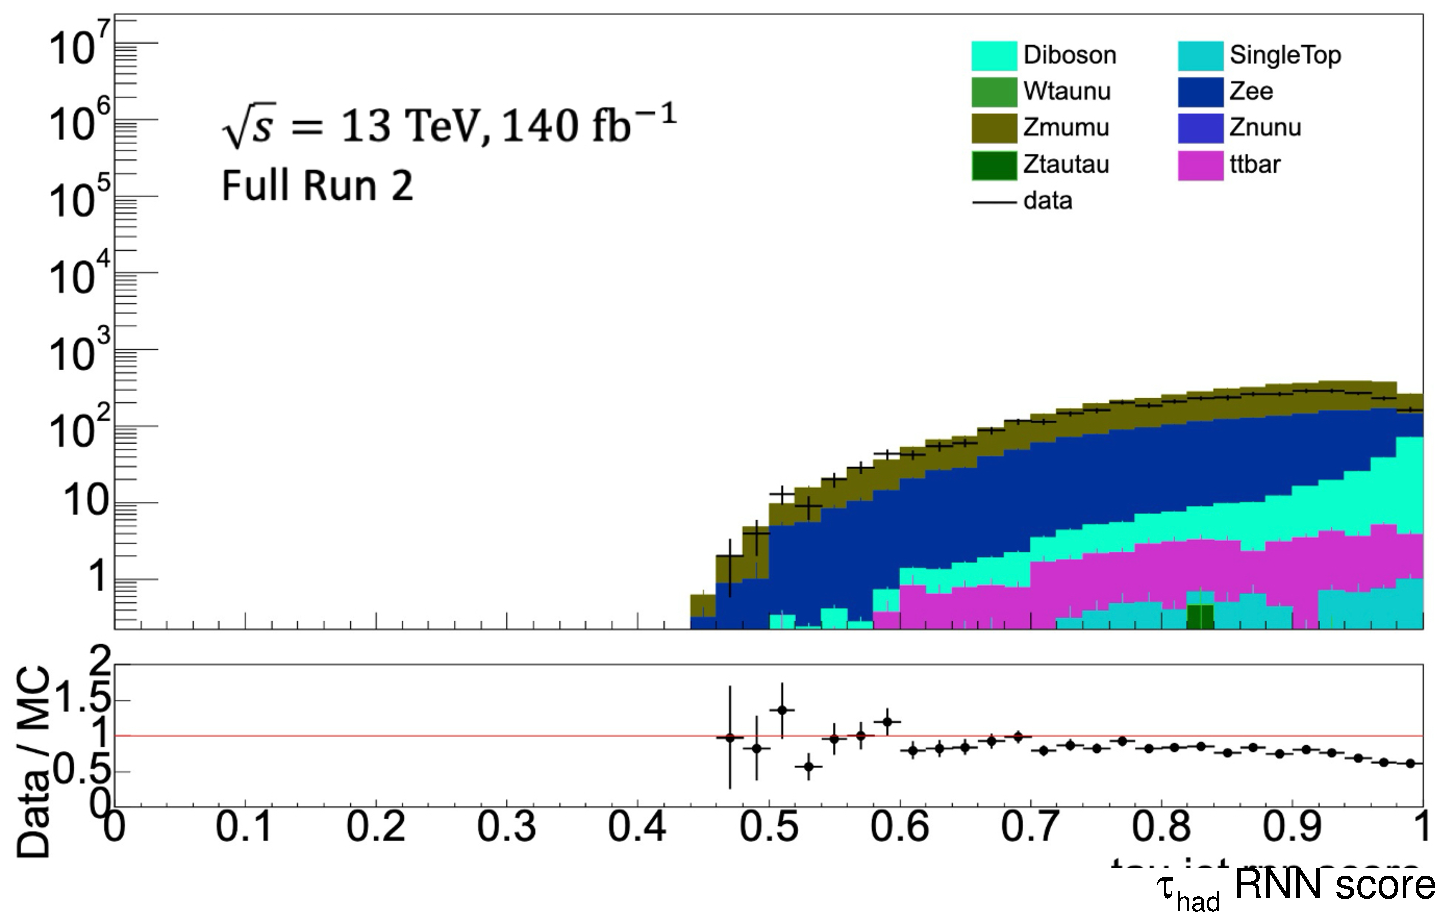
\includegraphics[width=\linewidth]{Figs/CH8/fake_tau_appendix/ZVR_1tau20GeV_score.pdf}
        \caption[]{$\pT^{\hadtau}>20~\GeV$}
    \end{subfigure}\hfill
    \begin{subfigure}{0.49\linewidth}
        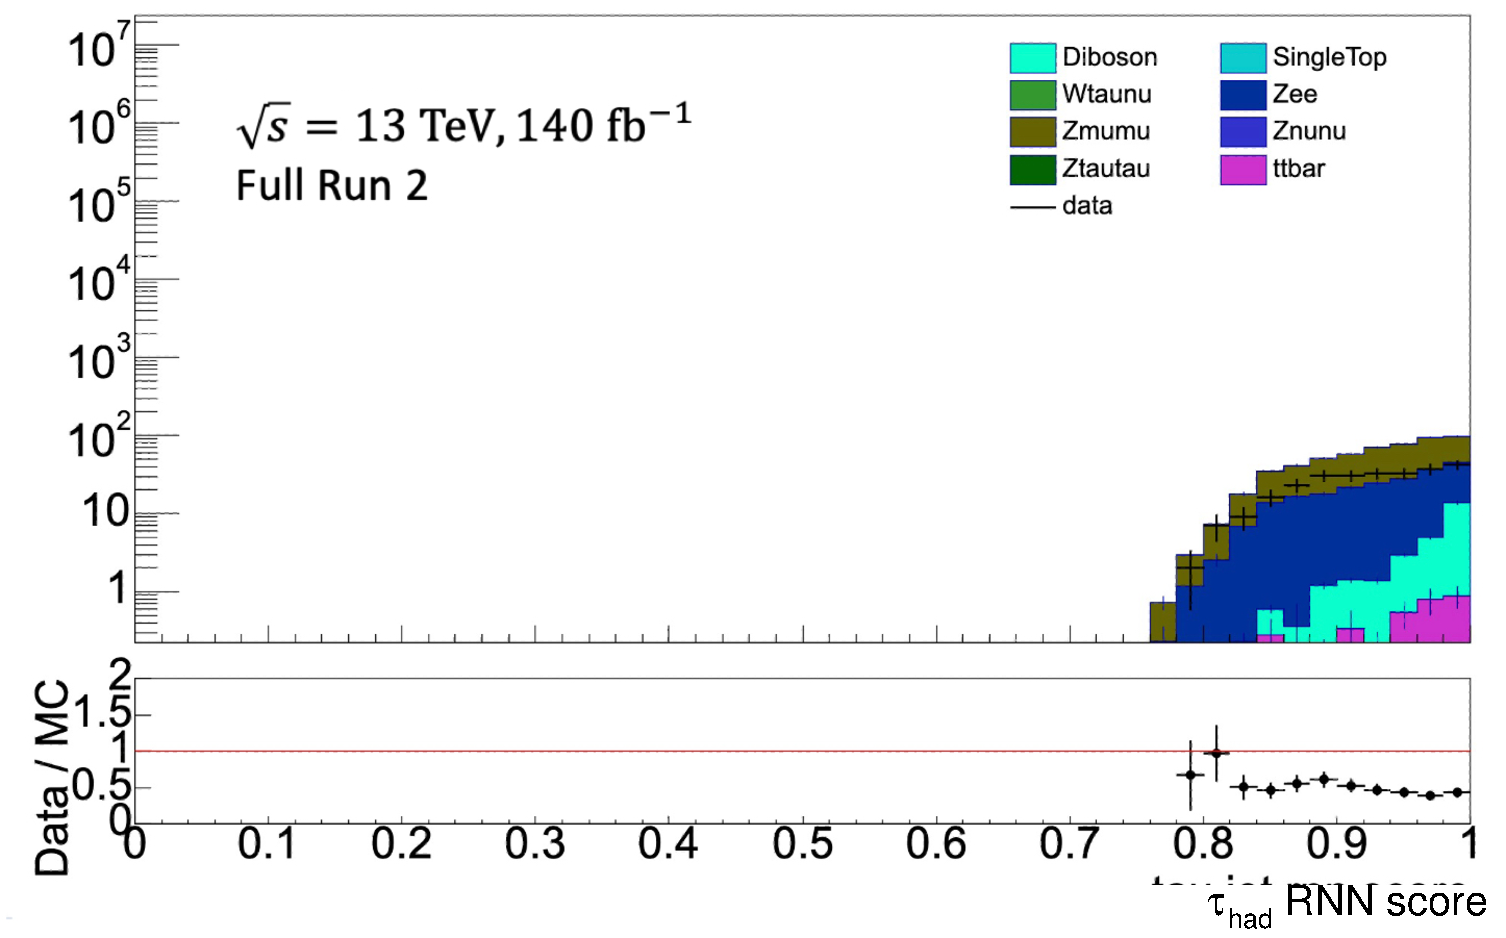
\includegraphics[width=\linewidth]{Figs/CH8/fake_tau_appendix/ZVR_1tau100GeV_score.pdf}
        \caption[]{$\pT^{\hadtau}>100~\GeV$}
    \end{subfigure}
    \caption[Tau-identification RNN distributions in the ZVR]{$\hadtau$-id RNN score in the regions of $\pT^{\hadtau}>20~\GeV$ (left) and $\pT^{\hadtau}>100~\GeV$ (right). Both figures use a loose $\hadtau$-id selection and a lower $\mT$ selection to observe the difference between high RNN score and low RNN score regions.}
    \label{fig:ch8_zvr_rnn}
\end{figure}
